\documentclass[a4paper,12pt,toc=flat]{report}
\usepackage{times}
\usepackage{sectsty}
\usepackage{graphicx}
\usepackage{multirow}
\usepackage{caption}
\usepackage{blindtext}
\usepackage[a4paper,total={6in,9in}]{geometry}


%\RequirePackage[left=6.1cm,top=2cm,right=1.5cm,bottom=2.5cm,nohead,nofoot]{geometry}

%\usepackage[a4paper,total={6in,8in}]{geometry}


\sectionfont{\fontsize{12}{15}\selectfont}
\subsectionfont{\fontsize{11}{12}\selectfont}


\usepackage{lipsum}% http://ctan.org/pkg/lipsum
\usepackage{titletoc}% http://ctan.org/pkg/titletoc
\titlecontents{chapter}% <section-type>
[0pt]% <left>
{}% <above-code>
{\bfseries\chaptername\ \thecontentslabel\quad}% <numbered-entry-format>
{}% <numberless-entry-format>
{\bfseries\hfill\ \contentspage}% <filler-page-format>


\linespread{1.5}

\usepackage[pagestyles]{titlesec}

\titleformat{\chapter}[display]
{\normalfont\huge\bfseries\centering}{\centering\chaptertitlename\ \thechapter}{20pt}{\Huge}
\titlespacing*{\chapter}
{0pt}{50pt}{40pt}

\pagenumbering{none}

\title{Online Car Rental System}
\author{ASWIN A K}
\date{August 2022}

\begin{document} 
	{\centering \bf \large
		 ONLINE CAR RENTAL SYSTEM\par
	}
	\begin{center}
		{\small PROJECT REPORT} \vspace*{17pt}
		\\ Submitted by\\
		\vspace*{17pt}
		{\bf ASWIN A K \\
			KMC21MCA-2008\\
			\vspace*{23pt}
			to}\\
		\vspace*{15pt}
		the APJ Abdul Kalam Technological University in partial fulfillment of
		the requirements for the award of the Degree\\
		\vspace*{9pt} of\\
		\vspace*{9pt} \textit{ Master of Computer Applications
		} 
		\vspace*{15pt}
		\begin{figure}[bph]
			\centering
			\includegraphics[width=0.3023\linewidth]{kmctlogo }
			
			\label{fig:kmctlogo}
		\end{figure}
		
		\bf{Department Of Management Studies  \& Computer Applications
			\vspace*{12pt}
			\\KMCT College of Engineering
			\vspace*{8pt}
			\\Kallanthode, NITC P.O, Kozhikode-673601}
		
	\end{center}
	\begin{center}
		\vspace*{6pt}NOVEMBER 2022
	\end{center}
	
	\thispagestyle{empty}
	\clearpage
	\pagebreak
	
	{\centering \bf \large
		DECLARATION\par
	}
	
	\vspace*{20pt}
	{\normalsize I undersigned hereby declare that the project report “{\bfseries 
			Online Car Rental System}”, submitted for partial fulfillment of the requirements for the award of degree of Master of Computer Applications of the APJ Abdul Kalam Technological University, Kerala is a bonafide
		work done by me under supervision of {\bf Mrs. Anjusha K}. This submission represents my ideas in my
		own words and where ideas or words of others have been included, I have adequately and accurately
		cited and referenced the original sources. I also declare that I have adhered to ethics of academic
		honesty and integrity and have not misrepresented or fabricated any data or idea or fact or source
		in my submission. I understand that any violation of the above will be a cause for disciplinary action
		by the institute and/or the University and can also evoke penal action from the sources which have
		thus not been properly cited or from whom proper permission has not been obtained. This report
		has not been previously formed the basis for the award of any degree. } \\
	
	
	\vspace{20pt}
	\begin{center}
		Place: Kallanthode \hspace*{14.5pt} \hfill  ASWIN A K  \\ \hfill\\ \hfill  \\
		\vspace*{10pt}
		Date: 24-11-2022 \hspace*{0pt} \hfill 
		\vspace{10pt}
		
		
		
	\end{center}
	
	\pagebreak
	
	
	\begin{center}
		
		\textbf{
			\vspace*{8pt}
			DEPARTMENT OF MANAGEMENT STUDIES \& COMPUTER
			\vspace*{8pt}
			APPLICATIONS\\
			KMCT COLLEGE OF ENGINEERING\\
			\vspace*{8pt}
			Kallanthode, NITC P.O, Kozhikode-673601
		}
		
		\begin{figure}[bph]
			\centering
			\hspace{-35}
			\includegraphics[width=0.8023\linewidth]{"kmct.png"}
			\label{fig:ksblogo}
		\end{figure}
	\end{center}
	{\centering \bf \large
		CERTIFICATE\par
	}
	\vspace*{10pt}
	This is to certify that the report entitled "{\bf 
		Online Car Rental System}"submitted
	by {\bf ASWIN A K (KMC21MCA-2008)}
	to the APJ Abdul Kalam Technological University
	in partial fulfillment of the requirements for the award of the Degree of Master of Computer
	Applications is a bonafide record of the project work carried out by her under our guidance and
	supervision. This report in any form has not been submitted to any other University or Institute for
	any purpose.
	
	\begin{center}\vspace*{20pt}
		Internal Supervisor \hspace*{0pt} \hfill  Project Coordinator
	\end{center}
	
	\begin{center}\vspace*{40pt}
		\hspace*{0pt} \hfill  Head Of The Department
	\end{center}
	\pagebreak
	
	\section*{\centering \bf \large ACKNOWLEDGEMENT}
	
	
	\vspace*{20pt}I would like to take this opportunity to extend my sincere thanks to people who helped me to make
	this project possible. This project will be incomplete without mentioning all the people who helped
	me to make it real.\\
	
	\hspace{12pt}First and foremost I thank {\bf Dr. Sabiq P V (Principal of KMCT College of Engineering)} who
	gave me all support to this project. I also thank {\bf Mr. Ajayakumar K K (Head of the Department,
		MCA)} for providing all the facilities and resources for my project. I would also like to express my
	gratitude towards {\bf Mrs. Remmya C B (Assistant Professor, MCA)}, Project Coordinator and  {\bf Mrs. Anjusha K (Assistant Professor, MCA)}, Project Guide for their
	continuous support, guidance and supervision without which the project wouldn’t have been a
	reality.  I would also take this
	opportunity to thank all my friends who took time out of their busy schedule to encourage, support
	and motivate me which has been the key reason for the successful completion of this project.\\ 
	
	Above all I thank God, the almighty for his grace without which it would not have been
	possible to complete this work on time.	
	
	
	
	\pagebreak
	\tableofcontents{}
	\pagebreak
		\chapter{INTRODUCTION}
	
	\hspace*{12pt}Gyms have become an essential part of our lives, providing the best exercise and body-building facilities to our society. Therefore, at the management end there are some necessary steps to maintain the records of every individual including a trainer, trainees, and staff but maintaining the records on paper is very difficult so, it is necessary to have a computerized system that manages all these issues. Gym Management Systems typically offer a wealth of solutions for every day operation, streamlining processes in a way that can enhance the customer experience. From online gym scheduling and automated billing to administrative tasks, the software pulls all data into one place so that you can run your business more efficiently. Gym management software is generally designed to streamline operations so that all of these tasks can be in one place. In a world where technological advances occur so quickly, it can feel like a challenge to keep up. But gym and fitness clubs can maximize business potential through gym management software. Simply, gym management software is a type of software that provides fitness businesses the functionality needed to manage all aspects of their business and efficiently operate their studio. Gym management software can also be referred to as club management software, fitness software, or gym scheduling software. Regardless of the nomenclature, these platforms all share similar feature sets and are used for the same purposes. Gym management software helps fitness owners and operators manage their class and trainer scheduling, keep track of their members, communicate with clients. Assuming clients enjoy the workouts and the sense of community at your studio, if the software is user friendly when they’re scheduling from a mobile app or on their computer, then they’ll continue to come back. The main objective of the Fitness Centre Management System is to manage the details of Fitness center, Fitness Master,  Member, Diets. It manages all the information about Fitness centre, Health, Diets. The project is controlling the administrator. The purpose of the project is to build an application program to reduce the manual work for managing the Fitness centre, Fitness Master, Health it tracks all the details about the Employee, Member, Diets. This project also incorporate bodymeasurements with the help of their photo using CNN Algorithm,and also find the nutrient content of food to capture an image then get the result.CNNs are powerful image processing, artificial intelligence (AI) that use deep learning to perform both generative and descriptive tasks, often using machine vision that includes image and video recognition, along with recommender systems and natural language processing (NLP). 
	\pagenumbering{arabic}
	\section{General Background}
	
	
	
	\hspace*{12pt}“Health care” Fitness center follows traditional fitness Center Managements, there is no guarantee for a computers or system to keep record of the Customers to be present. There is no suitable timetable for customers  and their workout is not arranged properly. So, there can be a clash in daily schedules. Since the records are in written documents, it is difficult to find the user names, Workout timings, summary etc. Administrator will be having a poor control over the Gym. They Using Paper work and direct human language communication to manage the Gym System will create problems, in terms of member records and their transactions which minimize the overall performance of the system and do not fulfill the requirements.  \\
	
	\pagebreak
	
	\section{Objective}
	\hspace*{12pt}In the AI based fitness management system provides a computer-based management system for keeping all records about Machinery, Members, and manage Fitness center, Fitness Master, Member, Diets, Workouts. This system helps the Owner and Admin to maintain large data about users and their daily plans in the gym center. This system is helping in creating reports and other record. The system is also suitable for users for an online profile my Gym Management system is the best option for it. It reduces and removes the manual and traditional workload. Administrator can easily add/ delete/ update/view each record on the computer. Mainly this project also incorporates bodymeasuremets with the help of CNN Algorithm and also predict the nutrient content of food with the help of image capture.  
	
	
	
	\hspace*{12pt}
	\pagebreak
	
	\chapter{\centering \bf \Large \hspace*{}SYSTEM ANALYSIS}
% \chapter{SYSTEM ANALYSIS}
        \\
        \\
        % 	\hspace*{130pt}{\centering \bf \Large SYSTEM ANALYSIS}
	\\
	\\
	\\
		
	
		\section{Existing system}
		\hspace*{12pt}{\normalsize
	The majority of the current automobile rental systems deal with customers in a conventional manner. The Car Rental System service will help users book a car for a fee specified. There was no clear web-based UI to help users rent the vehicle until now. They had to manually rent the vehicle through their offices. In this approach, tracking the details of booked and registered automobiles is done manually through paper work or an excel sheet. The customer needs to submit his licence and Aadhar card as proof of his citizenship and address. A user must visit the office to rent a car and make reservations for a car. Consumers want to rent a specific car, but frequently they do not see the car they are planning to travel in and wind up renting something else, ruining their trip. The current system has a hand-to-hand payment option. The customer must go and make a cash payment. Here, communication is only possible face-to-face. If the user needs to rent a car but is busy or has an emergency, he cannot do it using the conventional approach unless he travels there. In the system, customers can hire drivers for rent if they need to.In the modern digital era, where everything is available online, this strategy is no longer viable.
	\\
		
			
	\\
		\section{Proposed system}
	\hspace*{12pt}The online car rental system is a system for Symphony Car Rental, Kozhikode to automate the existing manual system. This system is a web-based application based on the concept of allowing customers to rent cars and drivers. The proposed system is being designed so that the work will become easier, faster, and more reliable than before. The major goal of the proposed system is to enhance and upgrade the existing systems with more efficiency, effectiveness, and also with low cost. 
	\\
	\hspace*{12pt}To access the homepage, admin must first log in. From the main page, the admin can add or update data. The system offers an admin-only part where vehicles and their details can be added, updated, or deleted. Admin can access the feedback and inquiry section to view user feedback and inquiries and respond to them. Admin can view available vehicles and drivers.The admin can view bookings made by customers and also can update their booking statuses.  
	
	To access the primary system, a user must first register and log in. Only after gaining access will they be able to select from a variety of car models and rent them out for a set period of time. With just a few clicks, customers can find everything on their internet-connected device. A user can quickly do a query in the system that is Speaking of the system's features, a user can choose among the various cars after logging in. The system shows the selected car's details when a selection has been made. The user must then enter information such as the number of days they plan to rent an automobile. Following these steps, the system verifies the rent. Customers can also rent drivers and can view profiles, select the driver and make contact. The Car Rental System takes care of all the inconveniences associated with traditional methods, which combine human interaction. No more phone calls or office visits, unlike current systems. Simply open the website, look through the cars, choose, and reserve. The customer would be given the best service available while saving time. Using this technique, the customer can easily obtain the car whenever they require it. Just a working internet connection is all they require. The system makes it simple for users to conduct inquiries. Inquiry is essentially an automated and computerised operation, which makes it much faster than it was in the past. Additionally, the client can leave feedback. Feedback is private information that can only be viewed by the admin.
	
		\\
		
			\vspace*{14pt}\hspace*{-16pt}{\bf Main activities of system are:} \vspace*{6pt}
			\\
				{\bf \hspace{-20pt} Login:}
				\\
	            Admin need to login to the web application by the already given username and password. User needs to register into the system first to avail the services available. This can be done by entering basic information like name, age, phone number, email address etc. After successful registration user can login to their account. Both Admin and Users can logout from the application.User can view and update their basic details given from Profile.
	            \\
	            		
	            			%\pagebreak
				{\bf \hspace{-20pt}Make Payments:}
				\\
	            Users can make payments of their rent amount.
	            \\
	            
	            
	            	{\bf \hspace{-20pt} Manage System:}
				\\
	            Admin can add new cars, update the details of cars such as brand, name, rent amount, etc., and delete cars. Admin and customers can view cars. Admin can change the home page information about the organisation so as to attract and give updated information to customers. An admin can manage users and drivers.admin to view the report of the month and helps the organisation to attain more knowledge about the most preferred vehicles among customers. This section contains the vital details that help to understand the business's growth.
	             \\
	           
	             
	              	{\bf \hspace{-20pt}Booking:}
				\\
	           Users can select their interesting cars to book and view the car details. Then select the number of days and kilometres to travel, and then calculate the rent amount. Then pay and book the vehicle.After booking vehicle the user can view their booking details.The user can also cancel the booking.The user may also hire a driver if they so want.
	             \\
	           
	            	
	             \\
	            
	            {\bf \hspace{-20pt}feedback and queries:}
				\\
	           The proposed system provides facilities for users to send feedback and queries about the website, services and organisation . Users can view the replies to their queries. The Admin has the option to view user feedback and queries and can send a response to received user queries.
	           \\

	             
	            
	           
	           
	          
	            
		
	          
	           	\section{Module Description}
	           \vspace*{6pt} \subsection{Admin}
	           	\hspace*{12pt}The admin is responsible for the overall management of this system. Admin needs to login to the application by the already given username and password. Main functions of admin include adding or updating information from home page. The system provides a section for admin to add, update or delete cars and its details like kilometres and category etc. Admin can view user feedback, enquiries and can reply to each from feedback and queries section. Admin can view available cars.The admin can view bookings made by customers and also can update their booking statuses.Rent information is immediately provided to the admin section when a customer chooses a certain car. They can also manage reservations and communicate with customers.
	           	\\
		\subsection{Customer}
	           	\hspace*{12pt}Customers who wish to rent a car or a driver should use this module. The customer must first register for a car rental using a username and password. When people log in after registering, they can access information about the vehicle, the driver, etc. The buyer can choose a car and, if necessary, a driver from the list of alternatives. The client may get in touch with them for additional questions.
	           	\\
	   \subsection{Driver}
	            \hspace*{12pt}Drivers must create an account with a username and password. They can include information about their driving history, licence, locations, etc. Users will be able to choose the best driver for them.The driver will be informed and provided contact information if a specific customer selects them.
	           	\\
	           \\
	           	\section{Feasibility Study}
	           	\hspace*{12pt}A feasibility study is a preliminary investigation conducted to ascertain and record the viability of a project. The purpose and logical goal of this study is to identify the advantages and disadvantages of a current or proposed system, as well as the possibilities and risks that exist in the surrounding environment. A feasibility study considers numerous limitations that the system should be operated and developed within. In order to establish whether the identified user's needs can be met using current software and hardware technologies, an estimate is made in this study, including the resource needed for implementation and expenses at the earliest possible time. Additionally, this analysis will determine whether the suggested system can be created within the available financial limits and will be cost-effective from a commercial standpoint. The study's findings are considered while deciding whether to move forward with the project or not.
	           	\\
	\subsection{Operational Feasibility}
	\hspace*{12pt}Operational feasibility examines how a project plan satisfies the requirements identified in requirements analysis phase of system development. It refers to the feasibility of the product to be operational. It mainly focuses on how the system satisfies the user needs. It helps in taking advantage of the opportunities and fulfills the requirements as identified during the development of the project. The new system or project can be used in day to day life which becomes more user friendly for the customer. This system is operationally feasible as it is very easy to operate. It helps the Shop owner to manage the operations in the shop. Also, the customers can easily view and book cars and drivers. 
	\\
		\subsection{Technical Feasibility}
	\hspace*{12pt}Technical feasibility study deals with the hardware and software and technology which are required to accomplish the user requirements in the system with in the allocated time and budget.The proposed system requires HTML, CSS, Python and MySQL platform   open source. Due to open source of languages it may not become complex to maintain and develop the system. The system can also be easily upgraded to the higher level with less effort and maintenance. This application can be easily used with their laptops or phones anywhere and also this application is very much user friendly. Hence the proposed work is technically feasible.
	\\
	\subsection{Economic Feasibility}
	\hspace*{12pt}Economic feasibility determines whether the proposed system is capable of generating profit for an organization. It involves costs incurred on the development team, estimated cost of hardware, feasibility study, and so on. This application was developed with the available resources. Since cost of input for the system is almost zero. The output of the website is always a profit for the user, and we see this as a service. This website doesn't cost any money from the users who are accessing it. Since the application can be accessed from any device with an internet connection, there is no need for specific hardware. Hence, it is economically feasible.
	\pagebreak
	
		
	\section{System Environment}
		
	\subsection{Developer Requirement}{
		
		{\bf 0.5.1.1 Hardware Requirement}{
			\begin{itemize}
				\item Processor : Intel Core i3 or above
				\item  RAM : 4 GB or above
				\item  Storage : 500GB Hard disk
			\end{itemize}
		}
		\\

	    \hspace*{-15pt}{\bf 0.5.1.2 Software Requirement}{
			\begin{itemize}
				\item  Operating system : Windows 8 or above 
				\item  Front end : HTML, CSS, BOOTSTRAP,JavaScript
				\item  Back end : MySQL
				\item  Languages : nodejs
				\item  IDE : VS code
				\item  Web browser : Google Chrome/Firefox
			\end{itemize}}
	    }
	\subsection{User Requirement}{
		    \begin{itemize}
			    \item  Any Smartphone/Computer/ Laptop
			    \item  Stable Internet Access
	        \end{itemize}
	}
	}
\newpage
	\section{Actors and their Roles}{
	\\
	\subsection{Admin}{
	The Admin is responsible for the overall management of this system.
	 \begin{itemize}
	\item Login
  \item Add/Update information in Home page
  \item View/manage all cars and Drivers
  \item View bookings made by Users 
  \item change booking status
 \item 	Add/Update/Delete the Cars 
 \item View/Respond to user feedback and queries
 \item View all users/view profile
  \item View Reports 
	\end{itemize}
	}
	\\
	 
	\\
	\\ \vspace*{11pt}
	
	\hspace*{-16pt} 
	\subsection{Customer}{
	    \hspace*{2pt} Customers can avail various services and features provided by the system after login.
	\begin{itemize}
	\item User Registration and Login
  	\item View/Update Profile
  	\item View all Cars and Driver
	\item Make bookings
	\item Cancel bookings
 	\item View car history
	\item View Booking
	\item Send feedback/queries and view reply

		
	\end{itemize}
	}
	
	
	\hspace*{-16pt} 
	
	\subsection{Driver}{
	
	    \begin{itemize}
	    
        \item Driver Registration and Login
        \item View/Update Profile
        \item View Booking Details
        \item Accept/Decline requests
        \item Upload Documents

	    
	\end{itemize}
	}
	
	
	\pagebreak
		
	}
		\chapter{\centering \bf \Large \hspace*{} METHODOLOGY}
    
        % 	\hspace*{130pt}{\centering \bf \Large METHODOLOGY}
	\\
	\\
	\\
        \section{Introduction}
        \\
        \hspace*{12pt}{ This project follows Agile methodology. Agile software development comprises various approaches to software development under which requirements and solutions evolve through the collaborative effort of self organizing and cross-sectional teams and their customers/end users. It advocates adaptive planning, evolutionary development, early delivery and continuous improvement and it encourage rapid and flexible response to change.}
\newpage
\section{UML Diagrams}
            \vspace{3mm}
        	\subsection{Use case Diagram}
        	\vspace{10mm}
        	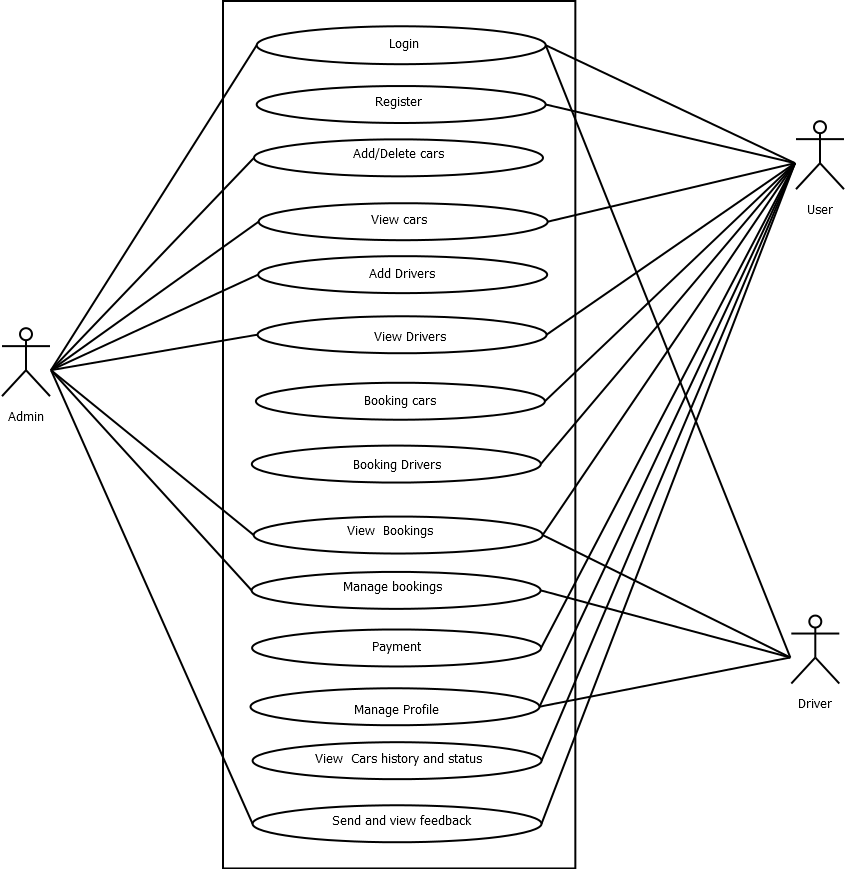
\includegraphics[width=16cm]{usecase.png}
        	\pagebreak
        	
        	\subsection{Class Diagram}
        	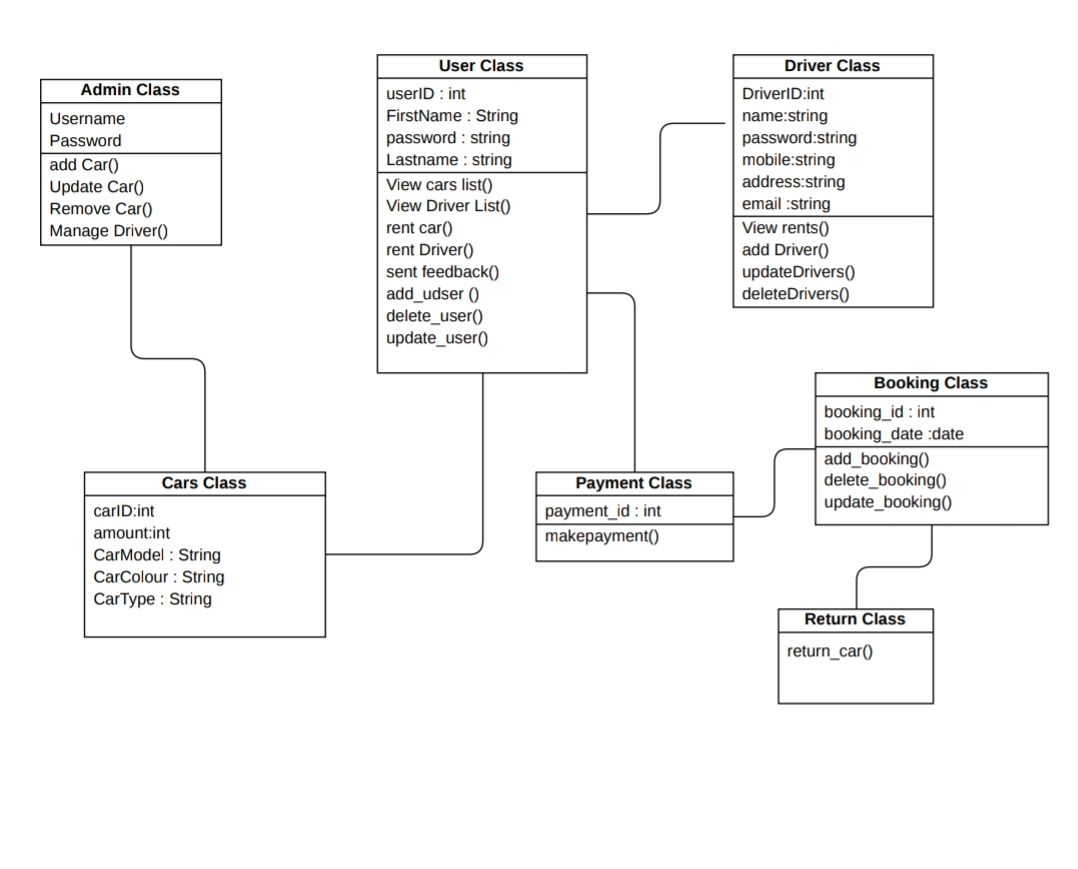
\includegraphics[width=14cm]{class.jpg}
        	
        	
        	\section{User Story}
        	\vspace{10mm}
	\begin{center}
		\fontsize{12}{12}\selectfont
		\begin{tabular} { | p {1.0 cm} | p {3 cm} | p {4 cm} |  p {4 cm} | }
			
			\hline\bf \vspace*{5pt} User story ID & \bf \vspace*{5pt}As a \textless Type of Users \textgreater & \bf \vspace*{5pt} I want to  \textless Perform	some task \textgreater &\bf \vspace*{5pt} So that I can \textless Achieve
			some goal \textgreater \\
			
			\hline
			1 & Admin, User,  Driver &	Home page&Home page for all users \\ \hline
			
			2 & Admin &Login & Admin access the system.\\ \hline
			
			3 & Admin &	Add car & Admin can Add Details of cars . \\ \hline
			4 &Admin &Add Drivers & Admin can add new drivers .\\ \hline
			
			
			5 & Admin &	Update car &Admin can update Details of cars . \\ \hline
			
			
			
			6 & User &	Login,Register&	user access the system.\\ \hline
			
			7 &User & Update profile  & Update user details.\\ \hline
			
			8 &User & Update documents & Upload document.\\ \hline
			9 &Admin & Get user & View all users and details.\\ \hline
			10 & Driver &login & Driver access the system .\\ \hline
			11 & Driver& Update details &	Update details of Driver. \\ \hline

			12 & Driver &Upload documents & Upload documents.\\ \hline
		    13 & User &	List Cars&View List of cars\\ \hline
		    14 & User &	Book Cars & Book cars from the list.\\ \hline
			15 & User& List Driver &View List of Drivers. \\ \hline	
			16 & User &	Book Drivers  & select Driver from the list\\ \hline
			17 & Driver & Receive booking& receive booking details\\ \hline
			18 & Admin & Booking Management & Admin can Manage Bookings. \\ \hline
			19 &User &	Feedback &send feedback.\\ \hline
			20 & Admin & feedback & view feedback and respond feedback.\\ \hline
			
			
			%21 &Admin &	homepage &  manage homepage.\\ \hline
		%	22 &User &	booking history &  View Booking history.\\ \hline
			
			
			
			
			
			
			
			
		\end{tabular} 
			\vspace*{12pt}
	\end{center}
		\pagebreak
	
	
	\section{ Product Backlog}
	
	\begin{tabular}{ | p {1.0 cm} | p {1.8 cm} | p {1 cm} |  p {1.2 cm} |  p {2.1 cm} |  p {2.0 cm} |  p {2.6 cm} | }
		\hline
		\centering	\bf User Story ID &
		\bf Priority
		(Low,High,
		Medium)   &
		\bf Size &
		\bf Sprint & 
		\bf Status (Planned,
		Progressed,
		Completed) &
		\bf Release Date & 
		\bf Release Goal \\
		\hline
		1& MEDIUM & 4 & &Planned & 04-09-2022 &Home page for all users\\ 
		\cline{1-3} \cline{5-7} 
		2& MEDIUM& 7 &                &Planned  & 08-09-2022 & Admin access the system\\ \cline{1-3} \cline{5-7} 
		3& HIGH & 4 &                   &Planned   & 10-09-2022 &Admin can add new cars\\ \cline{1-3} \cline{5-7} 
		4&MEDIUM  & 5 & {1}  &Planned  & 12-09-2022 &Admin can add new drivers\\ \cline{1-3} \cline{5-7}
		5&MEDIUM & 7 &                   &Planned    & 16-09-2022 &Admin can update details of cars \\ \cline{1-3} \cline{5-7}
		
		6& MEDIUM & 8 &	    				&Planned    & 21-09-2022 &User can register and login\\ \cline{1-3} \cline{5-7}  
			\hline
		7& LOW & 4 &                &Planned   & 23-09-2022 & User can do profile management  \\ \cline{1-3} \cline{5-7} 
		8& MEDIUM & 6 &      {2}       &Planned   & 25-09-2022 &User update documents  \\
		\cline{1-3} \cline{5-7} 
		
		9&  MEDIUM  & 12 & &Planned    & 30-09-2022 & View all users and details  \\ \cline{1-3} \cline{5-7}  \hline
	\end{tabular}
	
	\pagebreak
	\begin{center}
			\begin{tabular}{ | p {1.0 cm} | p {1.8 cm} | p {1 cm} |  p {1.2 cm} |  p {2.1 cm} |  p {2.0 cm} |  p {2.6 cm} | }
			\hline
			\centering	\bf User Story ID &
			\bf Priority
			(Low,High,
			Medium)   &
			\bf Size &
			\bf Sprint & 
			\bf Status (Planned,
			Progressed,
			Completed) &
			\bf Release Date & 
			\bf Release Goal \\
			\hline
			
			10&MEDIUM & 5 &                 &Planned   & 02-10-2022 & Driver access the system 	 \\ \cline{1-3} \cline{5-7} 
			11&  MEDIUM & 8 &       {2}               &Planned & 06-10-2022 &Update details of Driver\\
			\cline{1-3} \cline{5-7} 
			12&  MEDIUM & 4 &                    &Planned & 08-10-2022 &Upload documents\\
			\hline
			\cline{1-3} \cline{5-7} 
			13&  MEDIUM  & 6 &                   &Planned  & 10-10-2022 & View List of cars \\ \cline{1-3} \cline{5-7}
			
			
			
			14& HIGH & 7 &                   &Planned & 15-10-2022 &Book car from the list  \\ \cline{1-3} \cline{5-7}
			
			15& HIGH & 6 &        {3}             &Planned   & 18-10-2022 &View list of drivers \\ \cline{1-3} \cline{5-7}
			
			16& HIGH & 5 &     &Planned  & 21-10-2022 &select Driver from the list    \\ \cline{1-3} \cline{5-7}
			\hline
			17& HIGH  & 5 &                    &Planned   & 24-10-2022 &Receive booking details  \\ \cline{1-3} \cline{5-7}
			
			18& HIGH  & 5 &           {4}         &Planned   & 26-10-2022 &Admin can manage bookings  \\ \cline{1-3} \cline{5-7}
			
			19& MEDIUM  & 5 &                    &Planned   & 29-10-2022 &send  feedback  \\ \cline{1-3} \cline{5-7}
			
			20& MEDIUM  & 5 &                    &Planned   & 02-11-2022 &view and respond feedback  \\ \cline{1-3} \cline{5-7}
			
			%21& MEDIUM  & 3 &                    &Planned   & 03-11-2022 & Hompage management  \\ \cline{1-3} \cline{5-7}
			
			%	22& MEDIUM  & 4 &                    &Planned   & 06-11-2022 & View booking history  \\ \cline{1-3} \cline{5-7}
			\hline
		
			
		\end{tabular}
	\end{center}
	\pagebreak
	
	
		\section{Project plan}
	\begin{center}
		\begin{tabular} { | p {1 cm} | p {2 cm} | p {2 cm} |  p {2 cm} | p {1.5 cm} | p {3 cm} |  }
			
			\hline
			User story ID & Task name & Start date & End date & Days & Status
			Goal\\
			\hline
			1 & Homepage for all users & 02/09/2022 & 04/09/2022 & 2 & Planned\\ \hline
			2 &  Login of admin & 04-09-2022& 08/09/2022& 3 &Planned\\ \hline
            3& Add cars&08/09/2022 & 10/09/2022 & 2 &  Planned\\ \hline
			4 & Add drivers & 10/09/2022 & 12/09/2022 & 4 &Planned\\ \hline
			5 & Admin can update details of cars & 12/09/2022 & 16/09/2022 & 4 &  Planned\\ \hline
			6 & User register, login &  16/09/2022 & 21/09/2022 & 4 &  Planned\\ \hline
			7 &Update Profile details &21/09/2022 & 23/09/2022 & 2 &  Planned\\ \hline
			8 & Upload Documents &23/09/2022 & 25/09/2022 & 2 &  Planned\\ \hline
			9 & Get user details & 25/09/2022 &30/09/2022 & 2 &  Planned\\ \hline
			10 &Driver login &30/09/2022  &02/10/2022  & 2  &  Planned \\ \hline
			11&Update profile &02/10/2022  & 06/10/2022 &  4 &   Planned\\ \hline
		
			
				\end{tabular}
		\end{center}
	\pagebreak
	\begin{center}
\begin{tabular} { | p {1 cm} | p {2 cm} | p {2 cm} |  p {2 cm} | p {1.5 cm} | p {3 cm} |  }

\hline
User story ID & Task name & Start date & End date & Days & Status
Goal\\
\hline      	12& Upload documents & 06/10/2022  &08/10/2022   & 2  &  Planned \\ \hline
13& List cars &08/10/2022  & 10/10/2022  & 3 &  Planned \\ \hline
			14&Book cars & 10/10/2022 &15/10/2022  &4  & Planned\\ \hline
			15&List driver &15/10/2022  &18/10/2022 &3  &   Planned\\ \hline
			
				
	
			16&Select driver & 18/10/2022  &  21/10/2022 & 3 &  Planned\\ \hline
			17& Receive booking details & 21/10/2022 & 24/10/2022  &3  &   Planned\\ \hline
			18& Booking management& 24/10/2022  & 26/10/2022   &3  &  Planned \\ \hline
			19& Send feedback &  26/10/2022 & 29/10/2022 & 3 &   Planned\\ \hline
			20& View and Respond to feed back & 29/10/2022 & 02/11/2022 & 4  & Planned\\ \hline
		%	21& Homepage management & 02/11/2022   & 03/11/2022 & 3  & Planned\\ \hline
		%	22& View booking history & 03/11/2022   & 06/11/2022 & 4  & Planned\\ \hline
		
				\end{tabular}
		\end{center}
	\pagebreak
		
			\section{DATABASE DESIGN}	
	\subsection{Registration table}
	
	\\
	\begin{center}
		\begin{tabular} { | p {1 cm} | p {3 cm} | p {3 cm} |  p {3 cm} |  p {3 cm} | }
			
			\hline
			\centering
			\bf No. & \bf Name & \bf Type & \bf Constraints & \bf Description \\
			\hline
			1 & U\_id & INT & PRIMARY KEY &  Registration id of user\\ \hline
			2 & Fullname & VARCHAR(20) & NOT NULL &  Name of user\\ \hline
			3 & Gender & VARCHAR(6) & NOT NULL & Gender of user\\ \hline
			4 & Dob & date & NOT NULL & Date of birth of user\\ \hline
% 			5 & email & VARCHAR(35) & NOT NULL & email\_id of user\\ \hline
			5 & Phno & Int(12) & NOT NULL & Phone number of user\\ \hline
			6 & Address & VARCHAR(25) & NOT NULL &  Location of user\\ \hline
			7 & l\_id & INT & FOREIGN KEY &   Login id \\ \hline
			8 & Image& BLOB & NOT NULL & Image of the user\\ \hline
		\end{tabular} 
		\vspace*{12pt}
		\captionof{table}{Registration Table}
	\end{center}
	
% 	\pagebreak
		\subsection{login Table}
	
	\\
	\begin{center}
		\begin{tabular} { | p {1 cm} | p {3 cm} | p {3 cm} |  p {3 cm} |  p {3 cm} | }
			
			\hline
			\centering
			\bf No. & \bf Name & \bf Type & \bf Constraints & \bf Description \\
			\hline
			1 & l\_id & INT & PRIMARY KEY &   Login id \\ \hline
			2 & Email & VARCHAR(30) & NOT NULL &  Email id of user\\ \hline
			3 & Password & VARCHAR(100) & NOT NULL & Password of user\\ \hline
			4 & Usertype & VARCHAR(10) & NOT NULL & Type of user\\ \hline
		\end{tabular} 
		\vspace*{12pt}
		\captionof{table}{Login table}
	\end{center}
	
		\subsection{Car Table}
	
	\\
	\begin{center}
		\begin{tabular} { | p {1 cm} | p {3 cm} | p {3 cm} |  p {3 cm} |  p {3 cm} | }
			
			\hline
			\centering
			\bf No. & \bf Name & \bf Type & \bf Constraints & \bf Description \\
			\hline
			
			1 & car\_id & INT & PRIMARY KEY & id of car\\ \hline
			2 & Brand & VARCHAR(20) & NOT NULL & Brand of the car\\ \hline
			3 & Model & VARCHAR(10) & NOT NULL & model of car\\ \hline
			4 & Amount & INTEGER & NOT NULL & Rent amount\\ \hline
			5 & Fuel\_type & VARCHAR(10) & NOT NULL & fuel type of car\\ \hline
			6 & Reg\_no & VARCHAR(10) & NOT NULL & Registration number of car\\ \hline
			7 & Kms & INT & NOT NULL & Total kilometers runs\\ \hline
			8 & Status& VARCHAR(10) & NOT NULL & Status of car\\ \hline
			9 & Segment& VARCHAR(30) & NOT NULL & Segment of car\\ \hline
			10 & Transmission& VARCHAR(30) & NOT NULL & Transmission of car\\ \hline
			11 & No\_of\_seat& INT & NOT NULL & Number of seats in the car\\ \hline
			12 & Image& BLOB & NOT NULL & Image of the car\\ \hline



			
		\end{tabular} 
		\vspace*{12pt}
		\captionof{table}{Car table}
	\end{center}
	
	\pagebreak
		
		\subsection{Driver Table}
	\\
	\begin{center}
		\begin{tabular} { | p {1 cm} | p {3 cm} | p {3 cm} |  p {3 cm} |  p {3 cm} | }
			
			\hline
			\centering
			\bf No. & \bf Name & \bf Type & \bf Constraints & \bf Description \\
			\hline
			
			1 & Driver\_id & INT & PRIMARY KEY & id of Driver\\ \hline
			2 & Name & VARCHAR(20) & NOT NULL & Name of Driver\\ \hline
			3 & Address & VARCHAR(50) & NOT NULL & address of Driver\\ \hline
			4 & Gender & VARCHAR(6) & NOT NULL & gender of Driver\\ \hline
			5 & Experience & VARCHAR(10) & NOT NULL & Years of experience\\ \hline
			6 & Phno & INT(12) & NOT NULL & Phone number of Driver\\ \hline
% 			7 & email& VARCHAR(30) & NOT NULL & email\_id of Driver\\ \hline
			7& DOB& DATE & NOT NULL & DOB of Driver\\ \hline
			8 & Status& VARCHAR(10) & NOT NULL & Status of Driver\\ \hline
% 			10 & charge& INT & NOT NULL & Charge of Driver\\ \hline
            9 & L\_id & INT & FOREIGN KEY &   Login id \\ \hline

			
		\end{tabular} 
		\vspace*{12pt}
		\captionof{table}{Driver table}
	\end{center}
	\pagebreak
	
		\subsection{Booking Table}
	
	\\
	\begin{center}
		\begin{tabular} { | p {1 cm} | p {3 cm} | p {3 cm} |  p {3 cm} |  p {3 cm} | }
			
			\hline
			\centering
			\bf No. & \bf Name & \bf Type & \bf Constraints & \bf Description \\
			\hline
			
			1 & Booking\_id & INT & PRIMARY KEY & id of booking\\ \hline
			2 & Pic\_up\_date & DATE & NOT NULL & pic up date\\ \hline
			3 & Drop\_date & DATE & NOT NULL & drop date\\ \hline
			4 & Car\_id & INT & FOREIGN KEY & Car id\\ \hline
			5 & U\_id & INT & FOREIGN KEY & user id\\ \hline
			6 & Time & TIMESTAMP & NOT NULL & date time of booking\\ \hline
			7 & B\_status& VARCHAR(10) & NOT NULL & status of booking\\ \hline
			
            8 & D\_id & INT & FOREIGN KEY &   Driver id \\ \hline

			
		\end{tabular} 
		\vspace*{12pt}
		\captionof{table}{booking table}
	\end{center}
	
	
	
		
	
	
	

% 	\pagebreak
	
	
	\subsection{Payment}
	
	\\
	\begin{center}
		\begin{tabular} { | p {1 cm} | p {3 cm} | p {3 cm} |  p {3 cm} |  p {3 cm} | }
			
			\hline
			\centering
			\bf No. & \bf Name & \bf Type & \bf Constraints & \bf Description \\
			\hline
			1 & Pid & INT & PRIMARY KEY &  Id of payment\\ \hline
			2 & Bid & INT & FOREIGN KEY &  Booking id\\ \hline
			3 & Uid & INT & FOREIGN KEY & Id of user\\ \hline
			4 & Datetime & TIMESTAMP & NOT NULL & Date and time of payment\\ \hline
			5 & Amount & INT & NOT NULL & Amount to be paid\\ \hline
			6 & P\_status & INT & NOT NULL & Payment status\\ \hline
			
		\end{tabular} 
		\vspace*{12pt}
		\captionof{table}{Payment table}
	\end{center}

		\subsection{Feedback}
	
	\\
	\begin{center}
		\begin{tabular} { | p {1 cm} | p {3 cm} | p {3 cm} |  p {3 cm} |  p {3 cm} | }
			
			\hline
			\centering
			\bf No. & \bf Name & \bf Type & \bf Constraints & \bf Description \\
			\hline
			1 & Fid & INT & PRIMARY KEY & Id of feedback or query\\ \hline
			2 & Email & VARCHAR(45) & NOT NULL&Email Id of user  \\ \hline
			3 & Message & VARCHAR(200) & NOT NULL & Feedback message\\ \hline
			4 & Datetime & TIMESTAMP & NOT NULL & Date and time of feedback\\ \hline
			5 & Response & VARCHAR(200) & NULL & Reply for feedback or query\\ \hline
			
			
		\end{tabular} 
		\vspace*{12pt}
		\captionof{table}{Feedback table}
	\end{center}
	
	\subsection{Document table}

	\\
	\begin{center}
		\begin{tabular} { | p {1 cm} | p {3 cm} | p {3 cm} |  p {3 cm} |  p {3 cm} | }
			
			\hline
			\centering
			\bf No. & \bf Name & \bf Type & \bf Constraints & \bf Description \\
			\hline
			1 & Doc\_id & INT & PRIMARY KEY & Document id\\ \hline
			2 & Doc\_type & VARCHAR(45) &NOT NULL& Document type  \\ \hline
			3 & Doc\_img & BLOB & NOT NULL & Document image\\ \hline
			4 & U\_id & INT & FOREIGN KEY & User id\\ \hline
			
			
		\end{tabular} 
		\vspace*{12pt}
		\captionof{table}{Document table}
	\end{center}
	
	
	\pagebreak
	
	\section{FORM DESIGN}
	\subsection{Login page}
\hspace*{12pt}
	This is the login page for all the users of this system.
	\begin{figure}[bph]
	\begin{center}
		\includegraphics[width=1.1 \linewidth, height=0.7\textheight]{"login.png"}
	\end{center}
		\caption{Login page}
	\end{figure}

	\pagebreak
	

	\subsection{Registration page}
\hspace*{12pt}
	This is the Registration page for  the users of this system.
	\begin{figure}[bph]
	\begin{center}
		\includegraphics[width=1.2 \linewidth, height=0.7\textheight]{"signup.png"}
	\end{center}
		\caption{Registration page}
	\end{figure}

	\pagebreak
	
		\subsection{Admin page}
\hspace*{12pt}
	This is the admin page  of this system.
	\begin{figure}[bph]
	\begin{center}
		\includegraphics[width=1.1 \linewidth, height=0.7\textheight]{"admin.png"}
	\end{center}
		\caption{admin page}
	\end{figure}

	\pagebreak
	
		\subsection{Car list page}
\hspace*{12pt}
	This page is for the view and manage list of cars by admin.
	\begin{figure}[bph]
	\begin{center}
	\includegraphics[width=1.1 \linewidth, height=0.7\textheight]{"admin_carlist.png"}
	\end{center}
		\caption{car list page}
	\end{figure}

	\pagebreak
	
	
		\subsection{Driver list page}
\hspace*{12pt}
	This page is for the view and manage list of Driver by admin.
	\begin{figure}[bph]
	\begin{center}
		\includegraphics[width=1.1 \linewidth, height=0.7\textheight]{"admin_driver.png"}
	\end{center}
		\caption{Driver list page}
	\end{figure}

	\pagebreak
        	
        	
\subsection{Add Car page}
\hspace*{12pt}
	This page is for the  adding cars to the list  by admin.
	\begin{figure}[bph]
	\begin{center}
		\includegraphics[width=1.1 \linewidth, height=0.7\textheight]{"add_cars.png"}
	\end{center}
		\caption{add car page}
	\end{figure}

	\pagebreak
	
	
	
	\subsection{update car page}
\hspace*{12pt}
	This page is for update car details by admin.
	\begin{figure}[bph]
	\begin{center}
		\includegraphics[width=1.1 \linewidth, height=0.7\textheight]{"admin_update_car.png"}
	\end{center}
		\caption{update car page}
	\end{figure}

	\pagebreak
	
	\subsection{add driver page}
\hspace*{12pt}
	This page is for add new drivers to the list by admin.
	\begin{figure}[bph]
	\begin{center}
		\includegraphics[width=1.1 \linewidth, height=0.7\textheight]{"add_driver.png"}
	\end{center}
		\caption{add driver page}
	\end{figure}

	\pagebreak
	
	
		\subsection{ view all users page}
\hspace*{12pt}
	This page is for view  all users.
	\begin{figure}[bph]
	\begin{center}
		\includegraphics[width=1.1 \linewidth, height=0.7\textheight]{"admin_allusers.png"}
	\end{center}
		\caption{ view all users page}
	\end{figure}

	\pagebreak
	
	
	
			\subsection{ view user profile page}
\hspace*{12pt}
	This page is for viewing user profiles.
	\begin{figure}[bph]
	\begin{center}
		\includegraphics[width=1.1 \linewidth, height=0.7\textheight]{"admin_user.png"}
	\end{center}
		\caption{ view user profile page}
	\end{figure}

	\pagebreak
	
	
	
			\subsection{ view bookings page}
\hspace*{12pt}
	This page is for viewing bookings.
	\begin{figure}[bph]
	\begin{center}
		\includegraphics[width=1.1 \linewidth, height=0.7\textheight]{"admin_bookings.png"}
	\end{center}
		\caption{ view bookings page}
	\end{figure}

	\pagebreak
	
	
		\subsection{ view booking details page}
\hspace*{12pt}
	This page is for viewing booking details for a specific booking.
	\begin{figure}[bph]
	\begin{center}
		\includegraphics[width=1.1 \linewidth, height=0.7\textheight]{"admin_booking_details.png"}
	\end{center}
		\caption{ view booking details page}
	\end{figure}

	\pagebreak
	
	
		\subsection{ view feedback's page}
\hspace*{12pt}
	This page is for viewing feedback's.
	\begin{figure}[bph]
	\begin{center}
		\includegraphics[width=1.1 \linewidth, height=0.7\textheight]{"admin_feedback.png"}
	\end{center}
		\caption{ view feedback's page}
	\end{figure}

	\pagebreak
	
	
	
		\subsection{ send response page}
\hspace*{12pt}
	This page is for sending response to feedback's and queries.
	\begin{figure}[bph]
	\begin{center}
		\includegraphics[width=1.1 \linewidth, height=0.7\textheight]{"admin_response.png"}
	\end{center}
		\caption{ sending response page}
	\end{figure}

	\pagebreak
	
	
	
		\subsection{user page}
\hspace*{12pt}
	This page is the user page of the system.
	\begin{figure}[bph]
	\begin{center}
		\includegraphics[width=1.1 \linewidth, height=0.7\textheight]{"user.png"}
	\end{center}
		\caption{ user page}
	\end{figure}

	\pagebreak
	
		\subsection{View car list page}
\hspace*{12pt}
	This page is for viewing cars as a user.
	\begin{figure}[bph]
	\begin{center}
		\includegraphics[width=1.1 \linewidth, height=0.7\textheight]{"user_carlist.png"}
	\end{center}
		\caption{ car list page}
	\end{figure}

	\pagebreak
	
		\subsection{rent page}
\hspace*{12pt}
        This page is for selecting cars to rent and pay token amount.
	\begin{figure}[bph]
	\begin{center}
		\includegraphics[width=1.1 \linewidth, height=0.7\textheight]{"user_rent.png"}
	\end{center}
		\caption{ rent page}
	\end{figure}

	\pagebreak
	
	
		\subsection{select driver page}
\hspace*{12pt}
        This page is for selecting drivers to rent.
	\begin{figure}[bph]
	\begin{center}
		\includegraphics[width=1.1 \linewidth, height=0.7\textheight]{"user_driver.png"}
	\end{center}
		\caption{ drivers page}
	\end{figure}

	\pagebreak
	
		\subsection{Bookings page}
\hspace*{12pt}
        This page is for viewing  bookings of user.
	\begin{figure}[bph]
	\begin{center}
		\includegraphics[width=1.1 \linewidth, height=0.7\textheight]{"user_bookings.png"}
	\end{center}
		\caption{ booking page}
	\end{figure}

	\pagebreak
        	
        	
        	\subsection{View booking details page}
\hspace*{12pt}
        This page is for viewing  bookings details  of user.
	\begin{figure}[bph]
	\begin{center}
		\includegraphics[width=1.1 \linewidth, height=0.7\textheight]{"user_booking_details.png"}
	\end{center}
		\caption{ booking details page}
	\end{figure}

	\pagebreak
	
	
		\subsection{View documents page}
\hspace*{12pt}
        This page is for viewing  documents  of user.
	\begin{figure}[bph]
	\begin{center}
		\includegraphics[width=1.1 \linewidth, height=0.7\textheight]{"user_docs.png"}
	\end{center}
		\caption{ view documents page}
	\end{figure}

	\pagebreak
	
		\subsection{upload documents page}
\hspace*{12pt}
        This page is for uploading  documents  of user.
	\begin{figure}[bph]
	\begin{center}
		\includegraphics[width=1.1 \linewidth, height=0.7\textheight]{"user_upload.png"}
	\end{center}
		\caption{ upload documents page}
	\end{figure}

	\pagebreak
	
	
		\subsection{Inbox page}
\hspace*{12pt}
        This page is for viewing  responses and feedback's.
	\begin{figure}[bph]
	\begin{center}
		\includegraphics[width=1.1 \linewidth, height=0.7\textheight]{"user_inbox.png"}
	\end{center}
		\caption{ inbox page}
	\end{figure}

	\pagebreak
	
		\subsection{send feedback page}
\hspace*{12pt}
        This page is for users to send feedback .
	\begin{figure}[bph]
	\begin{center}
		\includegraphics[width=1.1 \linewidth, height=0.7\textheight]{"user_feedback.png"}
	\end{center}
		\caption{ send feedback page}
	\end{figure}

	\pagebreak
	
		\subsection{update profile page}
\hspace*{12pt}
        This page is for users to update their profile .
	\begin{figure}[bph]
	\begin{center}
		\includegraphics[width=1.1 \linewidth, height=0.7\textheight]{"user_update.png"}
	\end{center}
		\caption{ update profile page}
	\end{figure}

	\pagebreak
	
	
		\subsection{driver page}
\hspace*{12pt}
        This page is the driver page.
	\begin{figure}[bph]
	\begin{center}
		\includegraphics[width=1.1 \linewidth, height=0.7\textheight]{"driver_update.png"}
	\end{center}
		\caption{ driver profile page}
	\end{figure}

	\pagebreak
	
	
		\subsection{view driver documents page}
\hspace*{12pt}
        This page is for viewing  driver documents page.
	\begin{figure}[bph]
	\begin{center}
		\includegraphics[width=1.1 \linewidth, height=0.7\textheight]{"driver_docs.png"}
	\end{center}
		\caption{ view documents page}
	\end{figure}

	\pagebreak
	
		\subsection{upload documents page}
\hspace*{12pt}
        This page is for drivers to upload documents.
	\begin{figure}[bph]
	\begin{center}
		\includegraphics[width=1.1 \linewidth, height=0.7\textheight]{"driver_docs.png"}
	\end{center}
		\caption{ upload documents page}
	\end{figure}

	\pagebreak
	
			\subsection{booking of driver page}
\hspace*{12pt}
        This page is for viewing  bookings.
	\begin{figure}[bph]
	\begin{center}
		\includegraphics[width=1.1 \linewidth, height=0.7\textheight]{"driver_bookings.png"}
	\end{center}
		\caption{ driver's bookings page}
	\end{figure}

	\pagebreak
	
		\subsection{booking details of driver page}
\hspace*{12pt}
        This page is for viewing booking details of specific bookings.
	\begin{figure}[bph]
	\begin{center}
		\includegraphics[width=1.1 \linewidth, height=0.7\textheight]{"driver_booking_details.png"}
	\end{center}
		\caption{ driver's booking details page}
	\end{figure}

	\pagebreak
	
	
		\chapter{RESULT AND DISCUSSION}
	
	
	The project AI Based fitness center App was developed with proper planning and guidance. Agile methodology is used during the development of this project. Planning at each stage was done properly. Each sprint has been conducted as per protocol. Testing was performed at each stage of development. The project is  manage a health care fitness center edavannappara, through web application as well as android application.
	Web application is managed by the head of the fitness center of for adding details and solving their issues and manage the fitness center. Android application is used by Users so they can easily get to know about fitness.
\begin{figure}[!ht]
	\begin{minipage}{0.4\linewidth}
		\includegraphics[width=1.0\linewidth, height=0.4\textheight]{"C:/Users/user/Desktop/fitness center/pic/Screenshot_2022-05-06-22-35-43-61.jpg"}
		\caption{Nutreient content prediction}
	\end{minipage}
	\hfill
	\begin{minipage}{0.4\linewidth}
		\includegraphics[width=1.0\linewidth, height=0.4\textheight]{"C:/Users/user/Desktop/fitness center/pic/project/Screenshot_2022-05-03-17-27-06-51.jpg"}
		\caption{Nutreient content prediction }
	\end{minipage}
	\end{figure}
		\begin{figure}[!ht]
			\begin{minipage}{0.4\linewidth}
				\includegraphics[width=1.0\linewidth, height=0.4\textheight]{"C:/Users/user/Desktop/fitness center/pic/project/Screenshot\_2022-05-04-22-08-51-25.jpg	"}
				\caption{Body measurements}
			\end{minipage}
		
	
	
\end{figure}
	\newpage

	
	\chapter{CONCLUSION}
	
	
	The project "AI Based Fitness Center" put forward an effective way to communicate between fitness center and users,staffs in a perticular gym centers. Technology is improving day by day and everything is possible with our smartphone. This project aims at building an easy and effective way to manage a fitness center and interaction of user, This app brings a new opportunity for the people to interact with gym and take their bodymeasurements and nutrient content of food. It is really user friendly.
	
		\section{Future work}
		In the current application  is used mainly users pay the fees directly to the gym center. As future advancement, online payment optiopna are about to implementd. User can detect the nutrient content and their body measurements more accuratly from the image provided.
	
	\pagebreak

	


\section{References}

     \subitem[1]     W. Jia, R. Zhao, N. Yao, J. D. Fernstrom,M.
     H. Fernstrom, R. 
	J. Sclabassi and M. Sun, A food portion size measurement system
	 for image-based dietary assessment, in IEEE 35th Annual Northeast
		conference on Bioengineering, 2009.\\
\subitem[2] CNN Stanford University. [Online]. Available: http://cs231n.
		github.io/convolutional-networks/.\\ 
\subitem	[3] Center of Science in Public Interest. [Online]. Available:
	 https://cspinet.org/eating-healthy/why-good-nutrition-important. \\
	\subitem[4] P. Pouladzadeh, S. Shirmohammadi, and R. Al-Maghrabi, 
		Measuring calorie and nutrition from food image, IEEE Trans. 
		Instrum. Meas., 2014\\
\subitem	[5] P. Pouladzadeh, A. Yassine, and S. Shirmohammadi, FooDD: Food 
	detection dataset for calorie measurement using food images, in 
	Lecture Notes in Computer Science (including subseries Lecture 
	Notes in Artificial  Intelligence and Lecture
Notes in Bioinformatics), 2015.\\
\subitem	[6] R. A. Guler, N. Neverova, and I. Kokkinos, “Densepose: 
	Dense human pose estimation in the wild,” in Proceedings of the IEEE 
	Conference on Computer Vision and Pattern Recognition, 2018,
	 pp. 7297–7306.\\
\subitem	[7] https://colorlib.com/wp/free-bootstrap-admin-
		dashboard-templates/\\
\subitem	[8] https://www.taimoorsikander.com/registration-form-validation-in-
		android-studio/\\
\subitem	[9] https://www.geeksforgeeks.org/cardview-in-android-with-example/\\
\pagebreak
\subitem	[10] https://proandroiddev.com/avatarview-for-android-take-your-
	profile-images-to-the-next-level-2c0c6e06911c\\
\subitem	[11]https://www.androidhive.info/2011/10/android-login-and-
	registration-screen-design/\\
\subitem	[12] https://stackoverflow.com/questions/5944987/
		how-to-create-a-popup-window-popupwindow-in-android\\
	\subitem[13]https://code.tutsplus.com/articles/best-ecommerce-android-app-
		templates--cms-31887\\
	
\subitem[14]http://android-steps.blogspot.com/2015/08/profile-page-with-
circular-image-view.html?m=1\\
	\subitem	[15]https://www.kaggle.com/datasets\\
		
		

\pagebreak


 \section{Appendix}{
 }
	
\end{document}
